\documentclass[%
 reprint,
%superscriptaddress,
%groupedaddress,
%unsortedaddress,
%runinaddress,
%frontmatterverbose, 
%preprint,
%showpacs,preprintnumbers,
%nofootinbib,
%nobibnotes,
%bibnotes,
 amsmath,amssymb,
 aps,
%pra,
%prb,
%rmp,
%prstab,
%prstper,
%floatfix,
]{revtex4-1}

\usepackage{graphicx}% Include figure files
\usepackage{dcolumn}% Align table columns on decimal point
\usepackage{bm}% bold math

\begin{document}

\title{First Exclusive Measurement of Deep Virtual Compton Scattering off $^4$He: Toward the 3D tomography of nuclei}

\author{M. Hattawy, ...}
\affiliation{...}
\author{R. Dupr\'e}
\affiliation{Institut de Physique Nucl\'eaire d'Orsay, CNRS-IN2P3,\\ 
Universit\'e Paris-Sud, Universit\'e Paris-Saclay, 91406 Orsay, France.}

\date{\today}

\begin{abstract}
We report the first exclusive measurement of deeply virtual Compton scatterring 
(DVCS) off a nuclei with the CLAS detector at the Jefferson laboratory. The 
observed beam spin asymmetries are significantly larger than for proton, 
confirming expectations from plane wave impulse approximation. We present an 
extraction of the unique generalized parton distribution (GPD) of the spin-0 
helium in a completely model independent way. This result demonstrate the 
strength of the method and opens a new unique access into nuclei 3D structure 
in term of quarks and gluons.
\end{abstract}

\pacs{Valid PACS appear here}

\maketitle

%\section{Introduction}
% Now many letters do not put any sections. Maybe we should consider doing the same

The generalized parton distribution (GPD) framework developped in the past two decades
(Need a bunch of refs)~\cite{}
offers a unique access into hadron 3D structure through deeply virtual Compton
scattering (DVCS), depicted in figure~\ref{fig:DVCS} and other exclusive processes. Many measurements on the proton
at several energies have now be reported and have demonstrated the solidity of the
method~\cite{}. %To enhance a little -> CFF

Insert FIGURE DVCS nuclei
%\label{fig:DVCS}
\begin{figure}[htbp]
\caption{\label{fig:DVCS} Coherent DVCS}
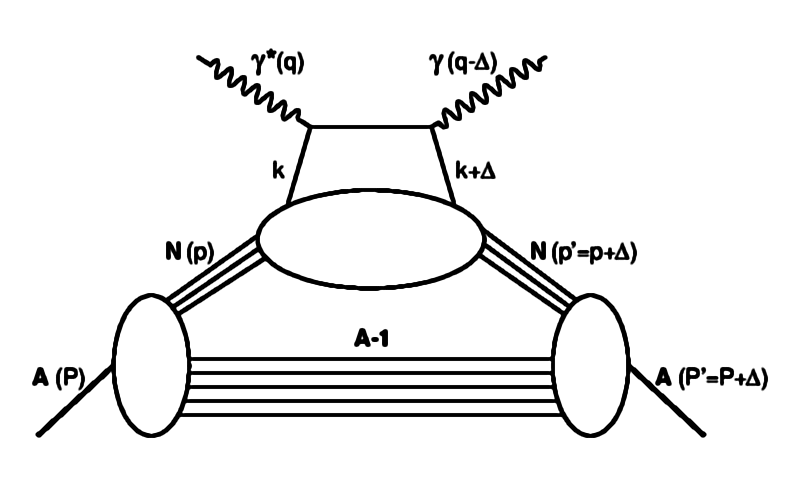
\includegraphics[width=8.6cm]{DVCS.png}
\end{figure}


At the same time, the partonic structure of nuclei has remained a mystery
for the past three decades, as we are still unable to explain properly the 
infamous EMC effect~\cite{}. First observed in 197X by the EMC 
collaboration, it describes the difference between the partonic structure of
free and bound nucleons. Understanding the source of this difference remains 
today a topic of active research~\cite{},
questionning our understanding of nuclei and their structure beyond protons
and neutrons~\cite{}. As studies based on inclusive measurements of the
effect seem to be too limited to tackle the question definitively, we can now
apply the GPD framework to study the nuclei in three dimensions and observe
the EMC effect in an unprecedented way.
%Elaborate on non nucleonic degrees of freedom and other interests of He DVCS

The measurement of DVCS on helium 4 is in this regard the perfect experiment for
several reasons. First, Helium 4 is of spin-0, such that a single GPD ($H$) is
necessary for the description of the DVCS at leading order. This feature allows for a
completely model independant extraction of the CFF from data that is impossible for 
protons and neutrons which need 4 GPDs, leading to complex underconstrained 
problems~\cite{}. Second, helium 4, while a small nuclei, is dense and experience 
already a significant EMC effect, while being simple enough that its nuclear
structure is very well known~\cite{} (Low energy struct, FF,...). Third, being 
light enough helium 4 can exit
a light target and be experimentally measured, insuring the exclusivity of the 
measurement. This point is especially important as we are probing with a 
multi-GeV interaction a nuclei bound by only a few MeV, this leads in the 
overwhelming majority of the cases to the incoherent break-up of the target.

%\section{Experiment}
The HERMES collaboration has measured nuclear DVCS~\cite{} without the 
possibility of separating the coherent and incoherent channels leading
to controversy in the interpretation of their results~\cite{}. We report
here our measurement of coherent DVCS off helium-4 at the Jefferson labortory
(JLab), while our results for the incoherent channel will be presented in
another paper~\cite{}. This experimental facility delivers a nearly 100\% duty factor, 6~GeV 
electron linear accelerator into three experimental halls. Our experiment
ran for 3 months in 2009 using the CEBAF Large Acceptance Spectrometer (CLAS).
This detector is covering about 2$\pi$ and is composed of drift chambers, Cherenkov counters, scintillator 
counters and an electro-magnetic calorimeter. It allows to detect accurately
electrons and provides a trigger for the experiment. It is complemented for DVCS experiments with
an inner calorimeter to detect the photons emitted at low angle and a solenoid
to keep the Moller electrons produced along the beam line to get into our detectors.

In order to insure the coherence of the process, we detect all the products
of the reaction. The electron is detected by the CLAS, using the drift chamber 
to reconstruct its trajectory and the combination of the Cherenkov counters
and electromagnetic calorimeter to 

we built a small and light 
radial time projection chamber (RTPC) depicted in figure~\ref{fig:rtpc} to 
detect the recoiling helium nuclei. this detector is placed directly ouside of 
our gaseous target filled with 6~atm helium. 
% to complete

\begin{figure}[htbp]
\caption{\label{fig:rtpc} RTPC description}
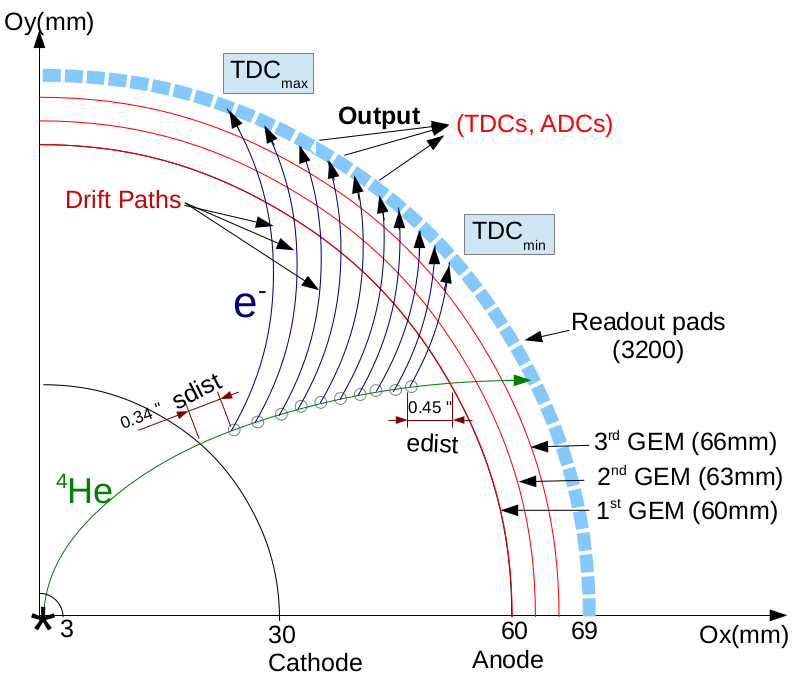
\includegraphics[width=8cm]{RTPC.png}
\end{figure}

%\section{DVCS Events Selection}

Detection, PID des particules.

\begin{figure*}[htbp]
\caption{\label{fig:exclu} Exclusivity cuts}
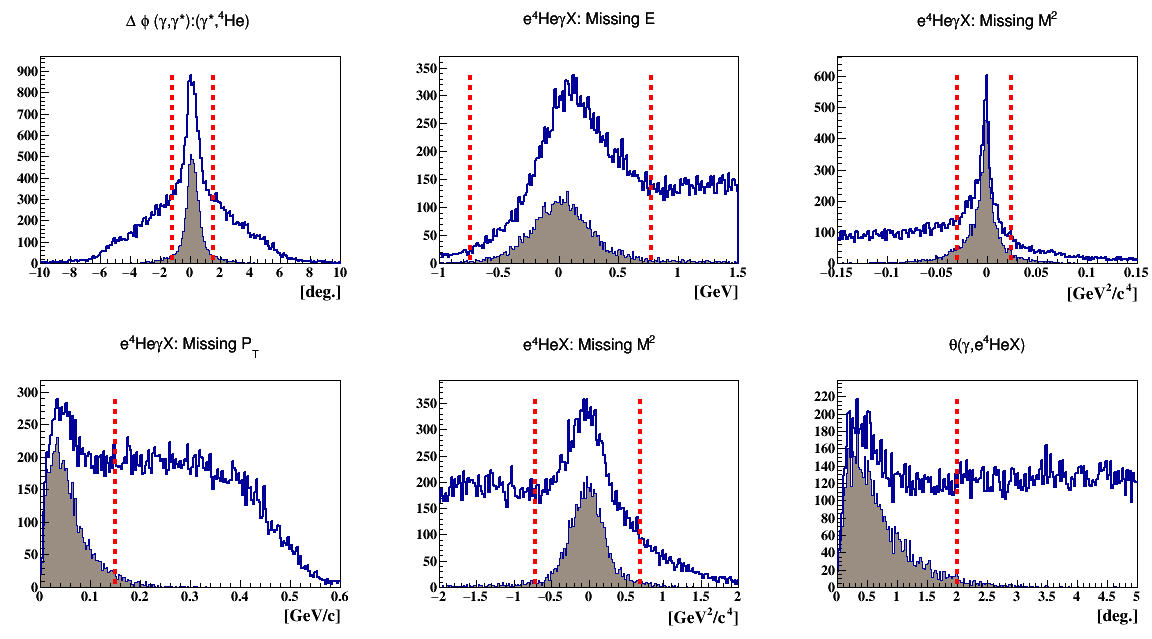
\includegraphics[width=17.2cm]{all_coh_exc_cuts.png}
\end{figure*}

We identified several background contributions to the DVCS process, in 
particular accidental events and exclusive deeply virtual $\pi^0$ production (DV$\pi^0$P). The accidental
events happen when an helium nuclei is mistakenly associated with our event, this 
possibility is suppressed by the limited phase space allowed but enhanced by the
low time resolution of the RTPC (~200 ns). We evaluated this contribution by
selecting events passing all our cuts but with particles originating from 
different verteces. With this method, we found this background to represent 
4.1\%. The DV$\pi^0$P events can easily be mistaken
with DVCS events when one of the two photons of $\pi^0$ decay is produced at
low energy in the laboratory frame. In order to estimate the importance of
this background, we developped an event generator DV$\pi^0$P 
that we calibrated to match our experimental yields. We used this generator together 
with a GEANT3~\cite{} simulation of our detection system to estimate the ratio 
of acceptance between measured DV$\pi^0$P and DV$\pi^0$P that would pass our 
DVCS selection cuts. This ratio obtained from simulation is then multiplied by 
the measured yield of DV$\pi^0$P events, indicating a contamination of XX to XX\%. 
%(We NEED a figure of that in the note!!!)

Systematic errors

%\section{Results}

Extraction of assymetries (figure~\ref{fig:assym})

\begin{figure*}[htbp]
\caption{\label{fig:assym} Assymetries}
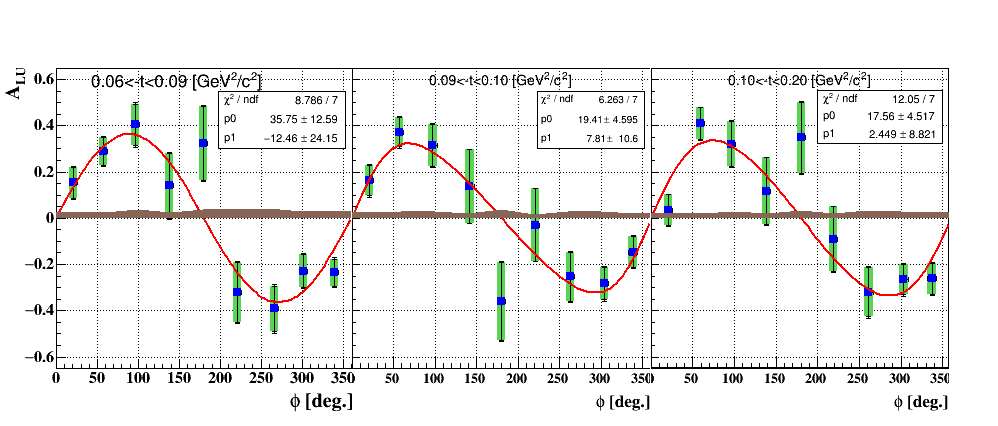
\includegraphics[width=14cm]{coh_alu_t_phi.png}
\end{figure*}


% This is mainly to compare to existing models
Generalized ratios (figure~\ref{fig:GenR})

\begin{figure}[htbp]
\caption{\label{fig:GenR} Generalized ratio}
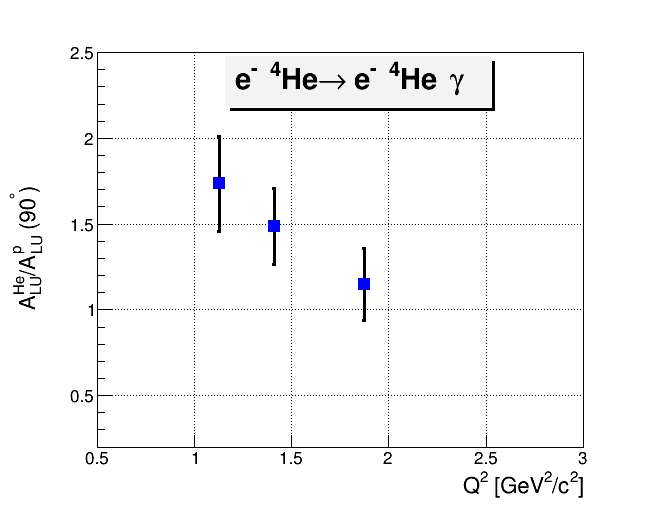
\includegraphics[width=7.5cm]{coh_emc_Q2.png}
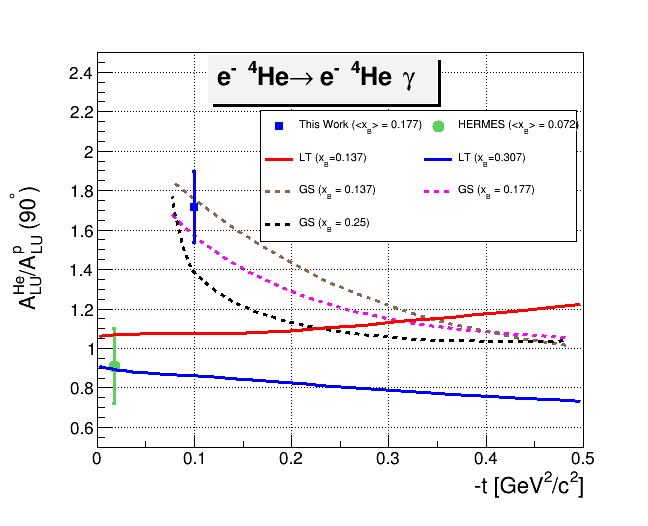
\includegraphics[width=7.5cm]{coh_emc_t.png}
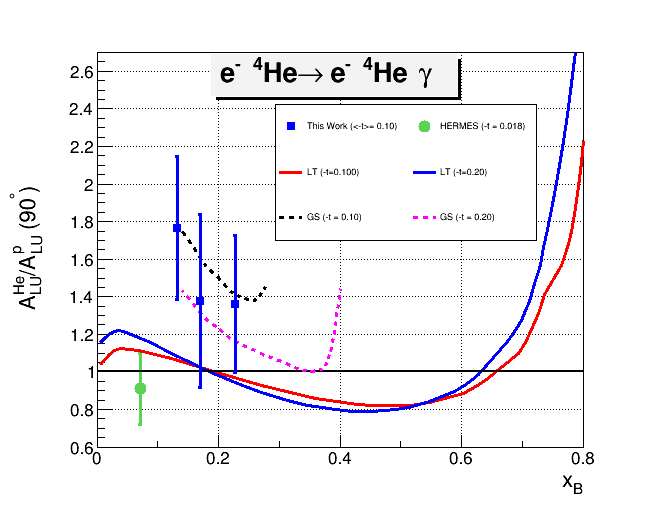
\includegraphics[width=7.5cm]{coh_emc_xB.png}
\end{figure}

\begin{figure}[htbp]
\caption{\label{fig:CFF} CFF extraction}
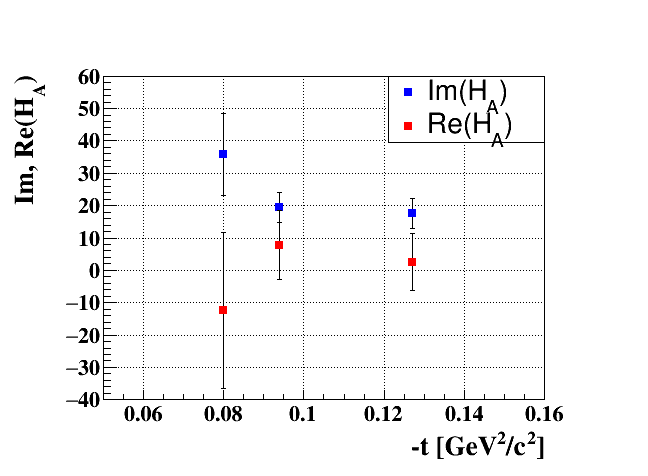
\includegraphics[width=8cm]{HA_t.png}
\end{figure}


Model independant extraction of H (figure~\ref{fig:CFF})


%\section{Summary}

Open new perspectives in nuclear physics, mention the 12 GeV program and the EIC

First fully exclusive measurement: very strong BSA, demonstrate the capability to extract GPDs even with limited statistics and kinematic compared to proton.

% If this is line > 400 this is probably getting too long!

\section*{Acknowledgments}
Guzey and Liuti

\section*{Bibliography}
Biblio

\end{document}

